\documentclass[onecolumn]{preport}
\usepackage[dvipdfmx]{graphicx}
\usepackage{listings}
\usepackage{color}
\usepackage{here}
\usepackage{url}
\graphicspath{{figs/}}
\title{クラウド基盤ソフトウェア課題レポート}
\author{480206515 知能機械情報学専攻 河村洋一郎}

\begin{document}

\pagestyle{empty}
\maketitle
\thispagestyle{empty}
\sloppy

\section{実験設定}
\subsection{実験に用いた計算機}
実験は手元のラップトップPC(ThinkPad P52S)で行った.計算機のスペックは
\begin{table}[htb]
  \begin{tabular}{c|l} \hline
    CPU & Intel(R) Core(TM) i7-8650U CPU @ 1.90GHz, 4コア8スレッド \\ \hline
    メモリ & 32GB DDR4 \\ \hline
    グラフィックボード &  Quadro P500 Mobile \\ \hline
  \end{tabular}
\end{table}
である.
\subsection{CPU仮想化なしの環境}
仮想化を行わない場合のホストOSはLinux (Ubuntu 18.04)を用いた.詳細なカーネルの情報は以下である.


\lstset{
  basicstyle={\ttfamily},
  identifierstyle={\small},
  commentstyle={\smallitshape},
  keywordstyle={\small\bfseries},
  ndkeywordstyle={\small},
  stringstyle={\small\ttfamily},
  frame={tb},
  breaklines=true,
  columns=[l]{fullflexible},
  %% numbers=left,
  xrightmargin=0zw,
  xleftmargin=3zw,
  numberstyle={\scriptsize},
  stepnumber=1,
  numbersep=1zw,
  lineskip=-0.5ex}
\begin{lstlisting}[language=c]
  $ uname -a
  Linux capricorn 5.3.0-61-generic #55~18.04.1-Ubuntu SMP Mon Jun 22 16:40:20 UTC 2020 x86_64 x86_64 x86_64 GNU/Linux
\end{lstlisting}

\subsection{CPU仮想化ありの環境}
仮想化を行った場合のホストOSはWindows10,仮想化にはVirtualBoxを使用し,ゲストOSにはLinux (Ubuntu 18.04)を用いた.(上記と同様)

また,仮想化マシンのメモリは、スワップが発生しないように16GBを割り当てた.

\subsection{行った実験}
行った実験は以下の3種類である.なお,今回は実験を行う途中に他のプロセスの優先度を変更したり止めることはせず,一般的なユースケースを想定してプログラムを実行した.

\begin {itemize}
\item フィボナッチ数を求める処理.\\ 漸化式$F_{n+2} = F_{n+1} + F_{n}$を用いて繰り返しで$F(n)$を求める$O(n)$の計算.同様の計算は10回行い平均と分散を求めた.
\item ローカルディスクにあるファイルへのread/write処理.\\ランダムな$N$文字をファイルに書き込み,その後書き込んだ文字を読み出す処理.同様の計算は10回行い平均と分散を求めた.
%% \item OpenGLのbench mark (glmark2 \cite{glmark2}) 
\end {itemize}

上2つの実験では,以下の条件で比較を行った.
\begin {itemize}
\item 仮想化環境でのCPU数が2,4,8に設定した場合で比較した(Hyper-Vは有効)\\ $\rightarrow$一般的なユースケースを想定するとHyper-Vがサポートされているなら有効にする場合が多いはずなので,Hyper-Vが有効になっている上でどの程度のCPU数を割り当てるのが良いのかを調べる目的で,このような設定にした
\item VirtualBoxの設定でHyper-Vを有効にした場合,仮想化アクセラレータなしの場合で比較した(CPUの数は4)\\ $\rightarrow$Hyper-Vの効果を調べる目的で行った
  
\end {itemize}

作成したプログラムはgithubで公開している\cite{myrepo}.上記の1,2のプログラムは\url{https://github.com/ykawamura96/CloudSoftware/blob/master/software/01_fibonacchi.py}と\url{https://github.com/ykawamura96/CloudSoftware/blob/master/software/02_io.py}で,いずれもpythonを用いて作成し,組み込みのtimeモジュールを用いて時間を測定した.

\section{結果}
塗りつぶした範囲は,10回の試行での$\pm 1 \sigma$の範囲を示す.

\figref{fib_cpu}と\figref{io_cpu}では、Hyper-Vオンで固定し,割り当てるCPU数を変更して比較している。

\figref{fib_acc}と\figref{io_acc}では、割り当てるCPU数を固定し、Hyper-Vのオンオフを変更して比較している。

\subsection{フィボナッチ数を求める処理}
\begin{figure}[H]
  \begin{center}
    \begin{minipage}{0.49\columnwidth}   
      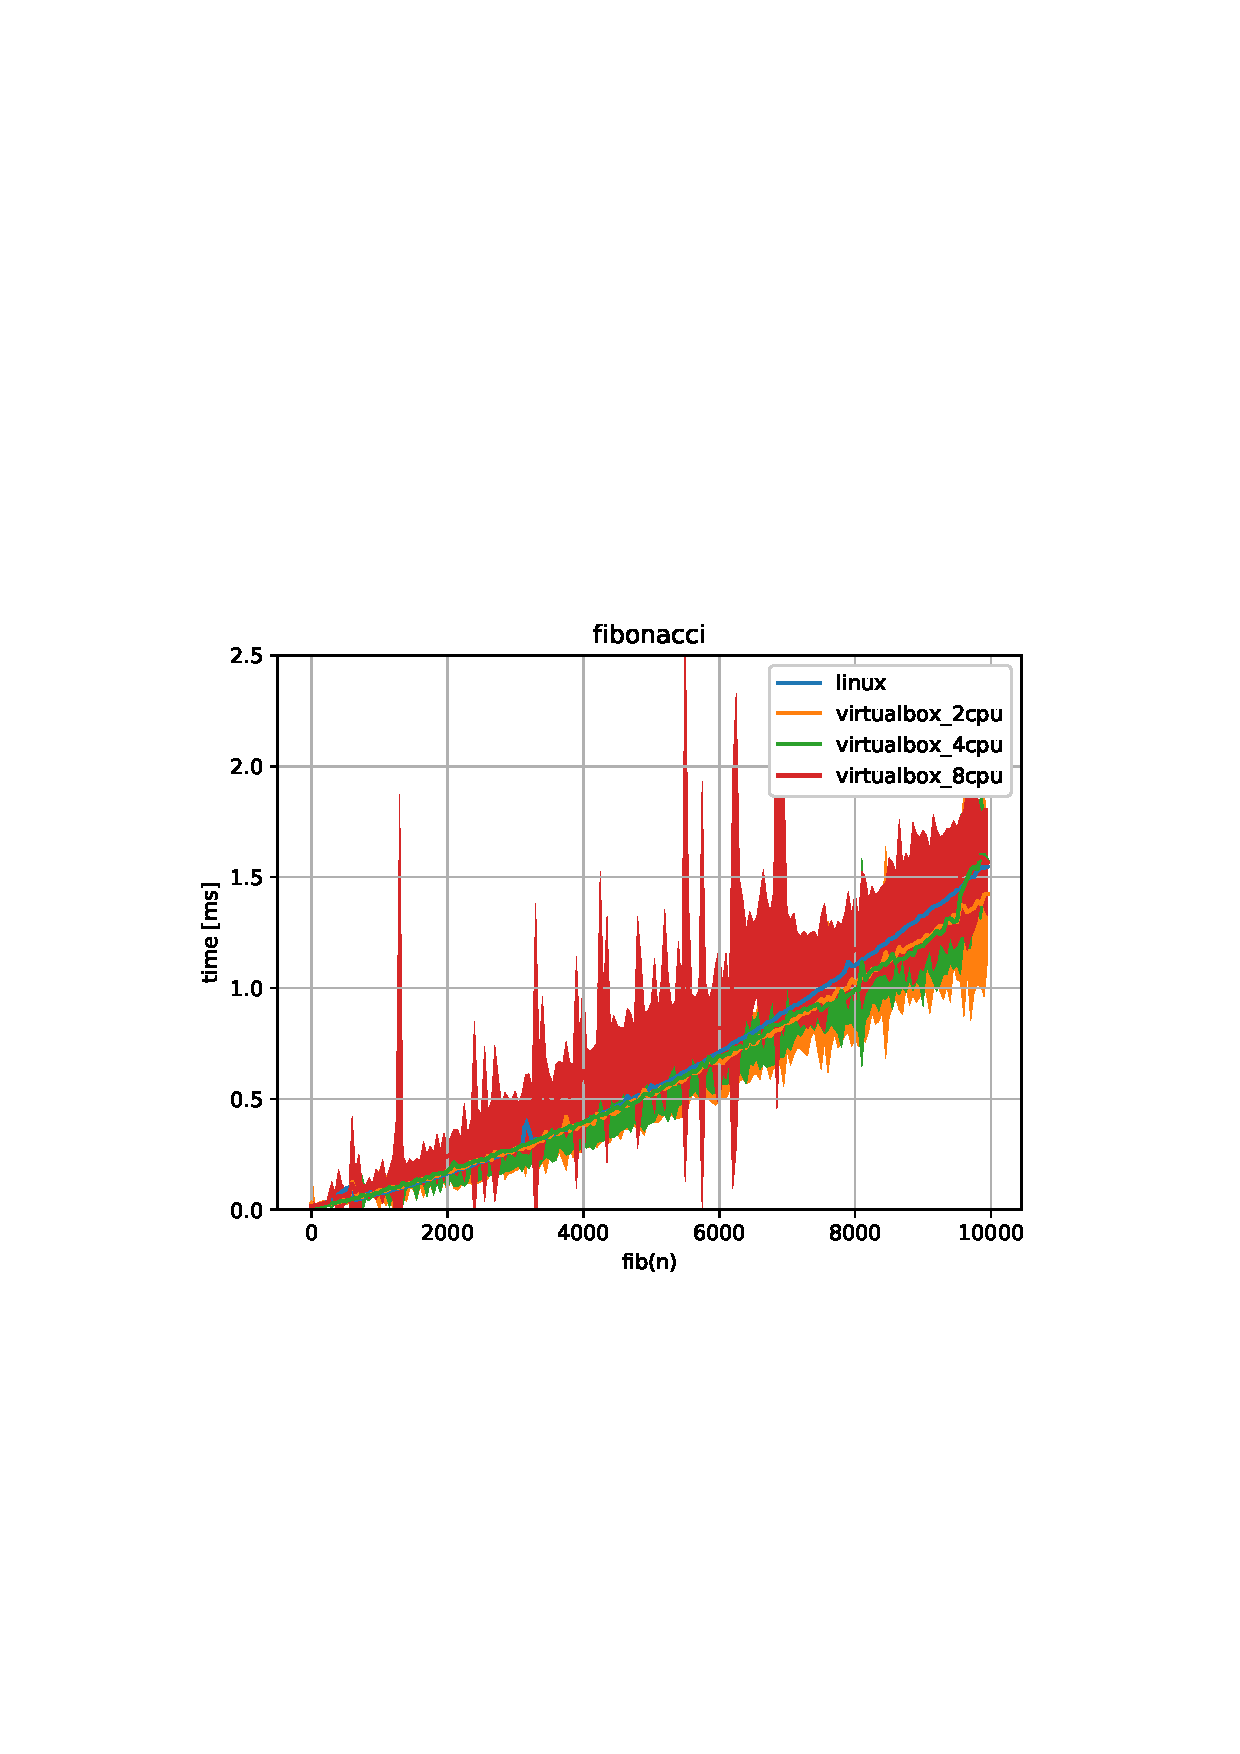
\includegraphics[width=\columnwidth]{_fib_cpu.pdf}
      \caption{フィボナッチ数: CPU数ごとの比較}
      \label{figure:fib_cpu}
    \end{minipage}
    %% \hspace{0.15\columnwidth}
    \begin{minipage}{0.49\columnwidth}
      \includegraphics[width=\columnwidth]{fib_acc.pdf}
      \caption{フィボナッチ数: アクセラレーションごとの比較}
      \label{figure:fib_acc}
    \end{minipage}
  \end{center}
\end{figure}

\subsection{I/Oを伴う処理}
\begin{figure}[H]
  \begin{center}
    \begin{minipage}{0.49\columnwidth}
      \includegraphics[width=\columnwidth]{io_cpu.pdf}
      \caption{I/O処理: CPU数ごとの比較}
      \label{figure:io_cpu}
    \end{minipage}
    %% \hspace{0.15\columnwidth}
    \begin{minipage}{0.49\columnwidth}
      \includegraphics[width=\columnwidth]{io_acc.pdf}
      \caption{I/O処理: アクセラレーションごとの比較}
      \label{figure:io_acc}
    \end{minipage}
    \label{figure:io}
  \end{center}
\end{figure}

%% \subsection{OpenGL}
%% glmark2を実行した結果以下のようになった.
%% \begin{table}[H]
%%   \begin{tabular}{c|c} \hline
%%     仮想化なし & 仮想化あり \\ \hline
%%     1149  & Segmentation Faultで完遂できず \\ \hline
%%   \end{tabular}
%% \end{table}
%% glmark2がvirtual boxで実行できない問題は,割り当てるビデオメモリをチューニングしたり,ビデオデバイスを変更するなど対策をしたものの治せず,今回のレポートには間に合わなかった.

%% ベンチマークの結果を以下に示す.

%% \subsubsection{仮想化なし}
%% \lstset{
%%   basicstyle={\ttfamily},
%%   identifierstyle={\small},
%%   commentstyle={\smallitshape},
%%   keywordstyle={\small\bfseries},
%%   ndkeywordstyle={\small},
%%   stringstyle={\small\ttfamily},
%%   frame={tb},
%%   breaklines=true,
%%   columns=[l]{fullflexible},
%%   %% numbers=left,
%%   xrightmargin=0zw,
%%   xleftmargin=3zw,
%%   numberstyle={\scriptsize},
%%   stepnumber=1,
%%   numbersep=1zw,
%%   lineskip=-0.5ex}
%% \begin{lstlisting}[language=c]

%%   $ glmark2
%%   =======================================================
%%   glmark2 2014.03+git20150611.fa71af2d
%%   =======================================================
%%   OpenGL Information
%%   GL_VENDOR:     NVIDIA Corporation
%%   GL_RENDERER:   Quadro P500/PCIe/SSE2
%%   GL_VERSION:    4.6.0 NVIDIA 440.100
%%   =======================================================
%%   [build] use-vbo=false: FPS: 988 FrameTime: 1.012 ms
%%   [build] use-vbo=true: FPS: 1481 FrameTime: 0.675 ms
%%   [texture] texture-filter=nearest: FPS: 1419 FrameTime: 0.705 ms
%%   [texture] texture-filter=linear: FPS: 1484 FrameTime: 0.674 ms
%%   [texture] texture-filter=mipmap: FPS: 1580 FrameTime: 0.633 ms
%%   [shading] shading=gouraud: FPS: 978 FrameTime: 1.022 ms
%%   [shading] shading=blinn-phong-inf: FPS: 980 FrameTime: 1.020 ms
%%   [shading] shading=phong: FPS: 920 FrameTime: 1.087 ms
%%   [shading] shading=cel: FPS: 1110 FrameTime: 0.901 ms
%%   [bump] bump-render=high-poly: FPS: 764 FrameTime: 1.309 ms
%%   [bump] bump-render=normals: FPS: 1479 FrameTime: 0.676 ms
%%   [bump] bump-render=height: FPS: 1703 FrameTime: 0.587 ms
%%   [effect2d] kernel=0,1,0;1,-4,1;0,1,0;: FPS: 1384 FrameTime: 0.723 ms
%%   [effect2d] kernel=1,1,1,1,1;1,1,1,1,1;1,1,1,1,1;: FPS: 980 FrameTime: 1.020 ms
%%   [pulsar] light=false:quads=5:texture=false: FPS: 1496 FrameTime: 0.668 ms
%%   [desktop] blur-radius=5:effect=blur:passes=1:separable=true:windows=4: FPS: 695 FrameTime: 1.439 ms
%%   [desktop] effect=shadow:windows=4: FPS: 858 FrameTime: 1.166 ms
%%   [buffer] columns=200:interleave=false:update-dispersion=0.9:update-fraction=0.5:update-method=map: FPS: 425 FrameTime: 2.353 ms
%%   [buffer] columns=200:interleave=false:update-dispersion=0.9:update-fraction=0.5:update-method=subdata: FPS: 627 FrameTime: 1.595 ms
%%   [buffer] columns=200:interleave=true:update-dispersion=0.9:update-fraction=0.5:update-method=map: FPS: 570 FrameTime: 1.754 ms
%%   [ideas] speed=duration: FPS: 1643 FrameTime: 0.609 ms
%%   [jellyfish] <default>: FPS: 783 FrameTime: 1.277 ms
%%   [terrain] <default>: FPS: 106 FrameTime: 9.434 ms
%%   [shadow] <default>: FPS: 1037 FrameTime: 0.964 ms
%%   [refract] <default>: FPS: 145 FrameTime: 6.897 ms
%%   [conditionals] fragment-steps=0:vertex-steps=0: FPS: 1522 FrameTime: 0.657 ms
%%   [conditionals] fragment-steps=5:vertex-steps=0: FPS: 1548 FrameTime: 0.646 ms
%%   [conditionals] fragment-steps=0:vertex-steps=5: FPS: 1619 FrameTime: 0.618 ms
%%   [function] fragment-complexity=low:fragment-steps=5: FPS: 1585 FrameTime: 0.631 ms
%%   [function] fragment-complexity=medium:fragment-steps=5: FPS: 1375 FrameTime: 0.727 ms
%%   [loop] fragment-loop=false:fragment-steps=5:vertex-steps=5: FPS: 1545 FrameTime: 0.647 ms
%%   [loop] fragment-steps=5:fragment-uniform=false:vertex-steps=5: FPS: 1595 FrameTime: 0.627 ms
%%   [loop] fragment-steps=5:fragment-uniform=true:vertex-steps=5: FPS: 1513 FrameTime: 0.661 ms
%%   =======================================================
%%   glmark2 Score: 1149
%%   =======================================================
%% \end{lstlisting}\label{figure:gl_linux}

\section{考察}
\subsection{仮想マシンに割り当てるCPUの数と処理時間の関係}
\figref{fib_cpu}, \figref{io_cpu}から
\begin{enumerate}
\item 処理時間について,CPU計算では仮想化あり/なしで計算時間に大きな差はない\\一方で,I/Oを伴う処理では仮想化ありでCPU数が4,8のとき若干仮想化のほうが遅い.CPU数が2の場合は,実行時間は仮想化なしの場合と大きな差はない.
  \begin{itemize}
  \item I/Oを伴う処理では処理時間の分散が大きいため,明確にI/Oを伴う処理が遅いとは言い難い
  \end {itemize}
\item 仮想化なしの場合より仮想化ありのほうが,処理時間の分散が大きい
\item CPU数が8 (計算機に乗っている物理的なCPU数と等しい)場合,実行時間のばらつきが顕著に大きい($\pm 1 \sigma$で塗りつぶされた範囲が大きい)
\end{enumerate}
という傾向があることがわかった.

授業で習った事項からは、Hyper-V等の仮想化支援機能を有効にした場合、仮想マシンでもそこそこ良い性能が得られるとが予想される。今回行った実験では、I/O処理について顕著に遅い(処理時間が1.5倍になるなど)とは言えなかった。よって、高々10KB程度のI/O処理や、fib(1000)を求める程度の計算ではVirtualMachineを使うことにより実用的な不都合が生じるとは考えにく区、十分実用的と言える。

一方でCPU数を8にしたときは、処理時間の分散が大きく、極端に処理時間が遅くなる場合があった。実際にEmacsなど体感の挙動も入力応答にラグを感じる瞬間があり不安定だった。

原因として、CPU数を8にすると、ユーザープロセスであるVirtualMachineAppの処理もプリエンプションされてしまうのではないかと考えた。特権命令を監視するVirtualMachineAppの処理に遅延が生じると、VirtualBoxで仮想化されたマシンの中での処理にも遅延が生じる。
しかし、この考え方だと、フィボナッチ数を求める処理(特権命令は走らないはず)でも処理時間に分散が生じることが説明できないため、要因は複数あると予想する。
実用的には、VirtualBoxにすべてのCPUリソースを与えると処理時間が安定しない場合があるので、避けたほうが良いということが言える。

\subsection{Hyper-Vと処理時間の関係}
\figref{fib_acc}, \figref{io_acc}からHyper-Vは性能向上に大きく寄与していることが分かる。Hyper-Vなしに比べて、CPU処理では概ね2倍、I/Oでは概ね3倍程度高速になっていて、BareMetalに遜色ない性能の発揮に寄与していることがわかる。
このことから、実用上Hyper-Vを有効にすることは、快適な仮想マシンライフを送る上で必要不可欠な機能であると言える。

%% \subsection{OpenGLのベンチマークについて}
%% 仮想マシンだとSegmentation Faultで完走できなかった。もう少し調べて弄ると直せるのかもしれないが、描画を伴う処理(やGPUでの計算)は仮想マシンで行おうとすると面倒な場合もあることがわかった。


\section{感想}
私が所属する研究室は、ロボットの研究室ですが、研究用途ではLinuxをBareMetalで使い、資料やスライドを作るためにwindows機を用いるという使わけをしていて、「windows機の仮想マシンは遅い」というイメージがなんとなくあったのですが、想像以上に高性能であり正直驚きました。

\bibliographystyle{junsrt}
\bibliography{p-report}

\end{document}
